\section{Problem Setup}

We assume a set of communicating components (actors) that interact
with each other.  These components may be user-defined (e.g.,
components that model an application that implements a distributed
protocol over a set of processes) or provided as an external entity
available to the application (e.g., a storage system or database).
Each component, regardless of whether they are user-defined or
system-provided, is equipped with a specification that governs its
allowed behaviors.  We formalize these specifications using the same
language we used in our PLDI'24 paper (i.e., LTL$_f$) that has a
natural representation as symbolic finite automata (SFA).  We have
refined our specification language so that they are now additionally
equipped with predicates that model the system's overall asynchronous
semantics.  For example, a read request performed by a client actor
may not be immediately serviced by the database.

\paragraph{Axioms and Specification} As a result of the inherently asynchronous
semantics of the systems we're modeling, component specifications must
capture how one message (aka event) might trigger another. For
instance, a specification that is associated with a coordinator that
manages the 2PC protocol might capture the property that a read
request that it receives initiates a chain of additional events or
messages as follows:
\begin{align*}
    \eff{ReadReq} \to \eff{GetReq} \to \eff{GetRsp}(v) \to
    \eff{ReadRsp}(v)
\end{align*}
\noindent where the payload of both $\eff{GetRsp}$ and $\eff{ReadRsp}$
contains the same value. These relationships are referred to as axioms
and are represented as individual temporal specifications for each
kind of message. For example, the specification $\phi_{\eff{ReadReq}}$
defined above, specifies that when the coordinator handles a
$\eff{ReadReq}$, it will send a $\eff{GetReq}$ to the database.

LTL$_f$ specifications for the 2PC coordinator and all participating
processes can be automatically extracted from their corresponding P
implementations, while specifications for the database or other
external components are provided manually.

\paragraph{Problem Setting}

Our tool takes a set of axioms $\Phi$ as described above and a
correctness property $A$ as input, and \emph{synthesizes} a program
$P$ that simulates a full test environment, generating requests to the
program under test, handling responses, and defining a linearizable
schedule among the actors comprising the system.  By removing ordering
constraints on message communication among components that are
explicit in the synthesized program, we essentially get a test
generator that relies on an external scheduler, similar to the
existing setup that uses the native $\Code{P}$ scheduler and monitor
to manage client process interactions, but which fully controls the
interaction between clients and external components.

\section{Motivating Example}

\begin{figure}[ht!]
    \centering
    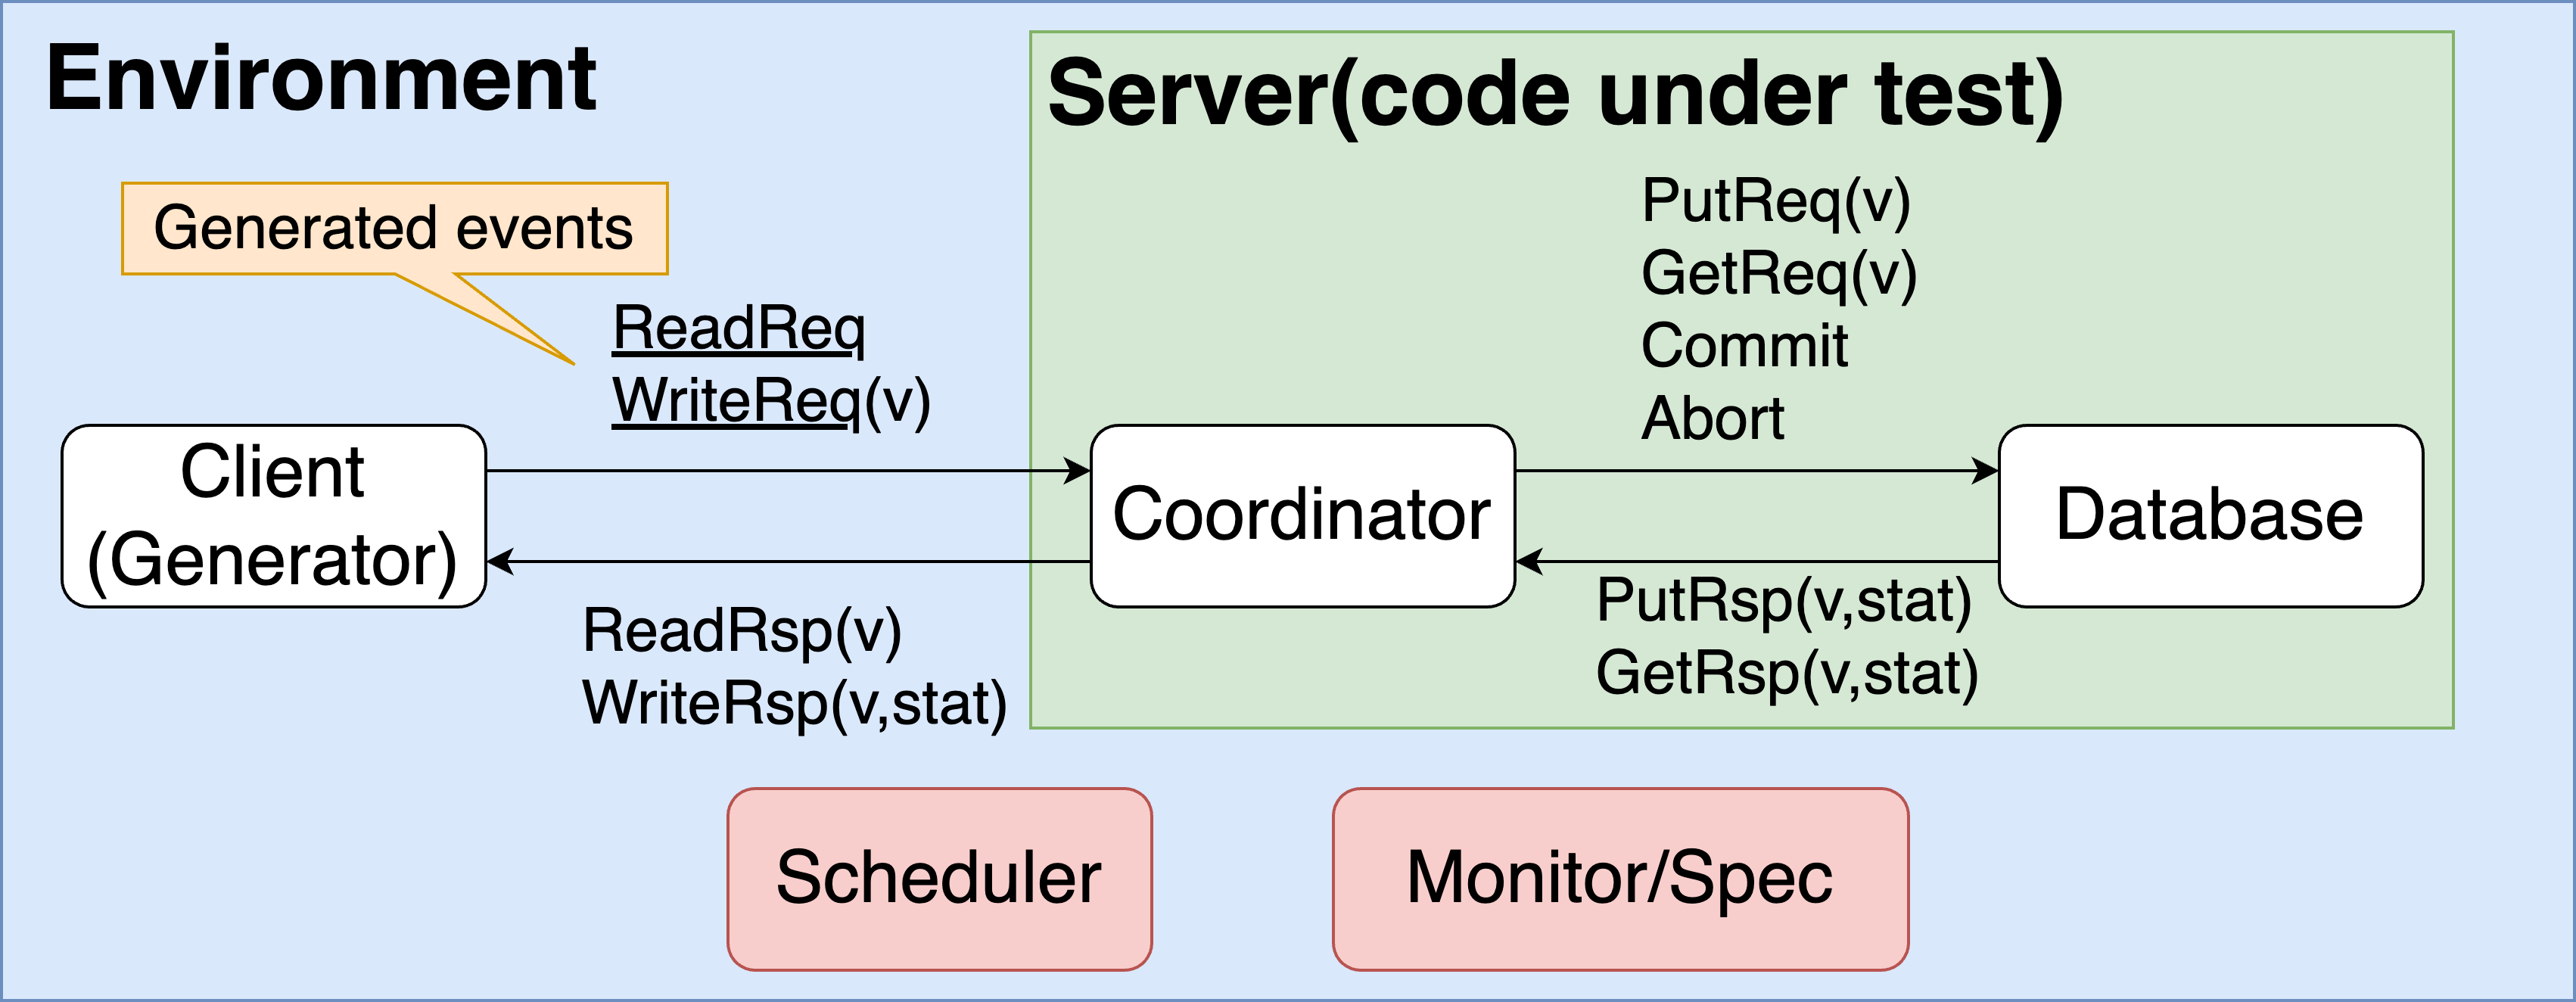
\includegraphics[width=0.75\linewidth]{figures/typed-guided-planing-example.drawio.png}
    \caption{A simple two-phase commit model.}
    \label{fig:ex-2pc}
\end{figure}

Following the above, we present a simplified two-phase commit model to
motivate our approach, as depicted in \autoref{fig:ex-2pc}. This model
comprises four components (machines):
\begin{enumerate} 
    \item The generator simulates user behaviors, enabling the sending
      and receiving of $\eff{Read/Write}$ messages for reading and
      writing values (specifically, the field $\Code{v}$ in the
      payloads). Furthermore, the response message (i.e., messages end
      with $\eff{Rsp}$) includes a Boolean field, $\Code{stat}$, which
      indicates the status code of the action performed.
    \item The implementation under test, illustrated in green in
      \autoref{fig:ex-2pc}, consists of two types of components: the
      coordinator and the database component. For clarity, we refer to
      the interactions between the coordinator and the database using
      $\eff{Put/Get}$ instead of read/write. The actual data is stored
      within the database components, while the coordinator retrieves
      this data and determines whether the updated information should
      be made persistent through $\eff{Commit}$ or $\eff{Abort}$
      messages.
    \item A scheduler determines the specific ordering of events
      produced by the generator.
    \item A monitor that determines that events observed by the
      coordinator and database are consistent with a global
      correctness property.
\end{enumerate}


\paragraph{Correctness Property} We aim to establish the correctness property $\exArw$,
which signifies strong consistency.\\[-.8em]

$\exArw$: \textit{Any read result (i.e., the $\Code{v}$ field of
  $\eff{ReadRsp}$) must equal the most recent successfully written
  value (i.e., when the $\Code{stat}$ field of $\eff{WriteRsp}$ is
  \Code{true}), which must hold for any write action that precedes
  a completed $\eff{Commit}$ action.}\\[-.8em]

The correctness property $\exArw$ can be formulated as a symbolic LTL
(Linear Temporal Logic) formula. However, the implementation may not
align with its requirements. For instance, the specifications
associated with database may only guarantee eventual consistency;
thus, a read result immediately following a successful committed write
might not reflect the written value, as the database may process the
read request out-of-order with the $\eff{Commit}$ message.

\paragraph{Environment and Generator} The environment encompasses
the elements required by the program under test (i.e., the
coordinator and database) during execution.  Our tool synthesizes
a program that models the behavior of the environment.  The behaviors
exhibited by this program are guaranteed to be consistent with
the specifications associated with the components being tested.

An important element of the environment is a generator that produces
\emph{generated events} (e.g., $\eff{WriteReq}$ and $\eff{ReadReq}$)
that need to be handled by the client program. The environment also
includes a scheduler that governs the order in which messages are
received by the actors comprising the coordinator, as well as a
monitor that check whether the \emph{observed} events are consistent
with the correctness property $\exArw$.

Although there are potentially infinitely many environment programs
that can be generated, we are particularly interested in identifying
those that result in the execution of the program under test to
violate the correctness property $\exArw$. This can occur when a
$\eff{ReadReq}$ message is generated, on a key that matches that of a
previous issued $\eff{WriteReq}$, which in turn precedes a generated
$\eff{Commit}$ message by the coordinator, but whose return value
payload does not match the payload of the $\eff{WriteReq}$.  An
example of a program that manifests this behavior, denoted as $e$, is
provided below. For simplicity, we assume there is only one
coordinator and one database, and therefore the source and destination
components (machines) of the messages are omitted.

\begin{minted}[xleftmargin=5pt, numbersep=4pt, linenos = true, fontsize = \footnotesize, escapeinside=??]{OCaml}
let (x: int) = ?$\mykw{random}$?(int) in
?$\mykw{assert}$? (x != -1) in
?$\mykw{generate}$? WriteReq x in
(* let (y1: int) = ?$\mykwCmt{observe}$? PutReq in *)
(* ?$\mykwCmt{assert}$? (y1 == x) in *)
(* let (y2: int), (s1: bool) = ?$\mykwCmt{observe}$? PutRsp in *)
(* ?$\mykwCmt{assert}$? (y2 == x && s1 == true) in *)
let (y3: int), (s2: bool) = ?$\mykw{observe}$? WriteRsp in
(* ?$\mykwCmt{assert}$? (y3 == x && s2 == true) in *)
?$\mykw{generate}$? ReadReq in
(* let () = ?$\mykwCmt{observe}$? GetReq in *)
(* let (y4: int) = ?$\mykwCmt{observe}$? GetRsp in *)
(* ?$\mykwCmt{assert}$? (y4 == -1) in *)
(* let () = ?$\mykwCmt{observe}$? Commit in *)
let (y5: int) = ?$\mykw{observe}$? ReadRsp in
(* ?$\mykwCmt{assert}$? (y5 == y4 && y5 != x) in *)
()
\end{minted}
This program can be considered as playing three distinct roles: as a
generator, a scheduler, and a monitor. Without the commented code, $e$
acts as a generator that  sends messages to the coordinator (on
lines $3$ and $10$) and receive responses (on lines $10$ and
$15$). This behavior is analogous to the following \Code{P} code.

\begin{minted}[xleftmargin=5pt, numbersep=4pt, linenos = true, fontsize = \footnotesize, escapeinside=??]{C}
var x: int;
value = choose(int);
assert(x != -1);
send coordinator, WriteReq, (source = this, v = x);
receive {
    case WriteRsp: ((y3: int, s2: bool)) {}
}
send coordinator, ReadReq, (source = this,);
receive {
    case ReadRsp: ((y5: int,)) {}
}
\end{minted}

We distinguish messages sent by the generator from other messages. The
former are ``announced'' using the $\mykw{generate}$ keyword, and it
is the responsibility of the execution environment in which this
program runs to provide the concrete payload of the message.  On the
other hand, the environment can also $\mykw{observe}$ other messages
and store the corresponding payload into variables (e.g., $y_3$ on
line $8$).

Moreover, if we include the commented code, the program gains a global
view (i.e., visibility of all events) and additionally functions as a
scheduler, dictating the order in which messages are received. For
instance, the $\eff{Commit}$ message (line $14$) is received after the
$\eff{GetRsp}$ message (line $12$), which is why the read value
remains the default value (i.e., $-1$) rather than the value that was
successfully written. The assertions in the commented code serve as a
monitor to ensure that the execution indeed produces a trace that
violates the correctness property $\exArw$.

The underlying intuition is that having a ``global view'' can lead to
more effective testing. Therefore, we first synthesize an environment
that acts as both a generator and a scheduler. Even if we later
``erase'' the invisible messages (i.e., those not sent or received by
the generator), the test remains more efficient.

